\documentclass[a4paper]{article}

\usepackage[english]{babel}
\usepackage[utf8x]{inputenc}
\usepackage{amsmath}
\usepackage{amsfonts}
\usepackage{graphicx}
\usepackage[]{algorithm2e}
\usepackage[colorinlistoftodos]{todonotes}

\title{CS 5785 -- Applied Machine Learning -- Lec.\ 15}
\author{Prof.\ Nathan Kallus, Cornell Tech\\Scribe: TBD}
\date{Oct.\ 24, 2017 }

\begin{document}
\maketitle

\section{Association Rule Mining: Market Basket Analysis}

We have seen some unsupervised learning methods by now:
\begin{itemize}
\item PCA, used mainly for dimensionality reduction.
\item $K$-Means, used for clustering.
\end{itemize}
In this lecture we will cover a new method of unsupervised learning called  \textit{Market Basket Analysis}, used for \textit{Association Rule learning/mining}.

\subsection{A Motivating Story}

Market Basket Analysis is a data mining technique used to study consumer purchases. It can help retailers understand what items are usually purchased together, develop marketing promotions, quantify purchasing trends for loyalty cards, manage inventory, etc.
\begin{figure}
\centering
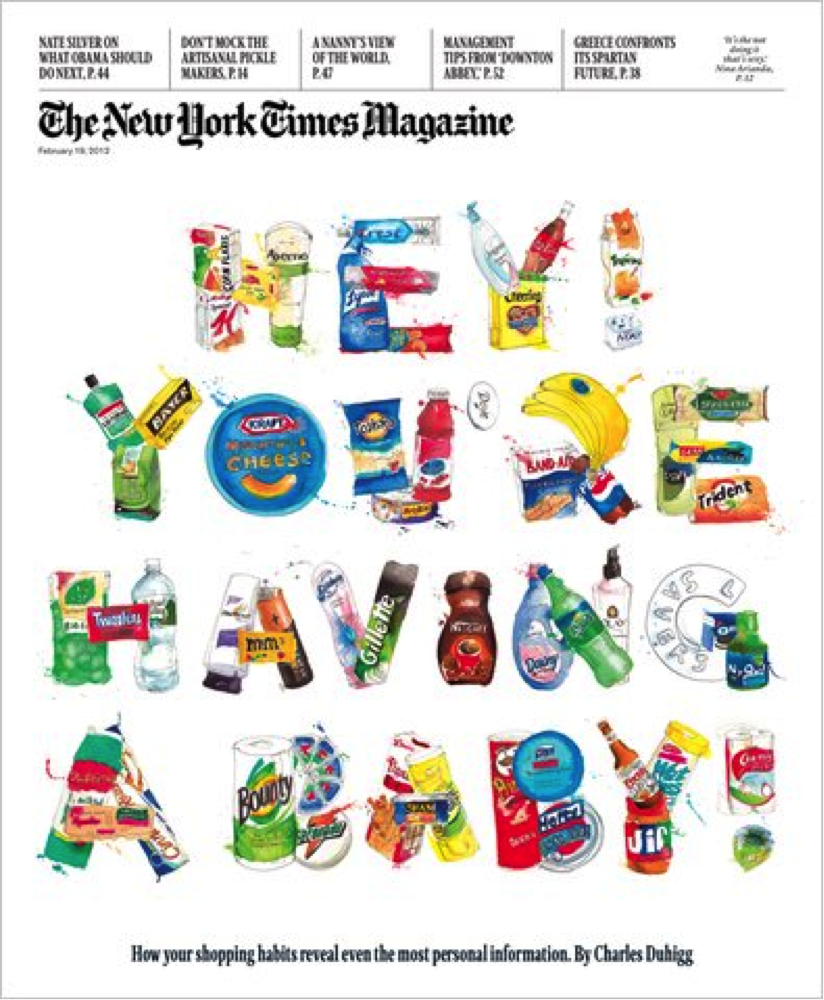
\includegraphics[width=0.5\textwidth]{TargetMarketBasket.png}
\caption{\label{fig:target} A New York Times Magazine article about Target's Market Basket Analysis scandal.}
\end{figure}

Data scientists at Target generated a minor scandal through a provocative use of market basket analysis; see Figure \ref{fig:target}.  Their algorithms predicted, based on a set of items bought by a certain household, that there was a pregnant woman in the house. Following that conclusion they mailed baby and pregnancy related promotions to the household. The father got angry and complained to Target that no one in his family is pregnant and that they should stop sending them such promotions. Later, the father found out that his teenage daughter was pregnant. After this incident, Target continued to use market basket analysis, but cleverly camouflaged their curated advertising pages amongst a set of standard promotions to avoid scaring off customers or creating a fear of being watched.

\begin{figure}
\centering
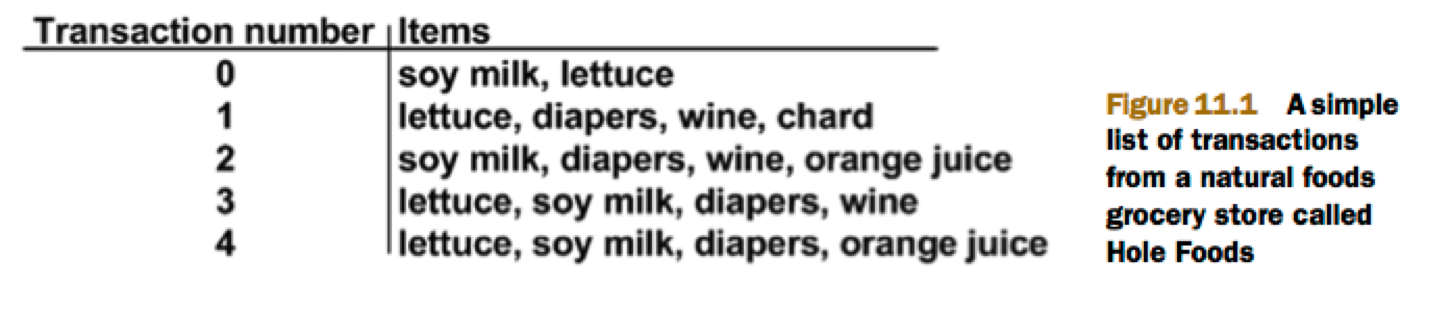
\includegraphics[width=1.0\textwidth]{ItemsetExamples.png}
\caption{\label{fig:itemsets} Example itemsets from course book}
\end{figure}

\subsection{Support and Confidence}

\newenvironment{definition}[1][Definition]{\begin{trivlist}
\item[\hskip \labelsep {\bfseries #1}]}{\end{trivlist}}

\begin{definition}
\underline{Support} of an itemset is the precentage of the dataset containing this itemset.
\end{definition}

For example, in the dataset shown in Figure \ref{fig:itemsets} the support for the itemset \{soymilk\} is $\frac{4}{5}$, since \textit{soymilk} appears in $4$ out of the $5$ itemsets. The the support for the itemset \{soymilk, diapers\} is $\frac{3}{5}$, since \textit{soymilk} and \textit{diapers} appear together in $3$ out of the $5$ itemsets.

\begin{figure}
\centering
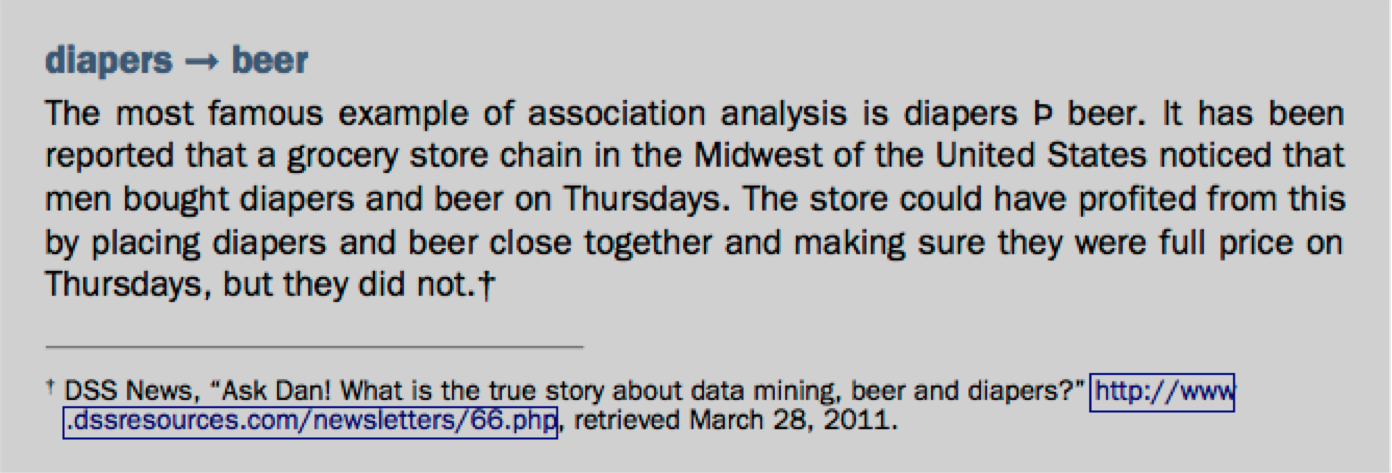
\includegraphics[width=1.0\textwidth]{DiapersBeers.png}
\caption{\label{fig:diapersBeer} Most common associative rule example}
\end{figure}

\begin{definition}
\underline{Confidence} of an association rule $\{A\}\rightarrow\{B\}$ is:
$$\frac{support(\{A, B\})}{support(\{A\})}$$
\end{definition}

For example, the confidence of the association rule $\{diapers\}\rightarrow\{wine\}$ based on the dataset described in Figure \ref{fig:itemsets} is:
$$conf(\{diapers\}\rightarrow\{wine\})=\frac{support(\{diapers, wine\})}{support(\{diapers\})}$$
$$\Downarrow$$
$$conf(\{diapers\}\rightarrow\{wine\})=\frac{\frac{3}{5}}{\frac{4}{5}}=\frac{3}{4}=0.75$$
Meaning that in $75\%$ of the transactions in the dataset that contain \textit{diapers} our rule is correct, i.e., the itemsets contain also \textit{wine}.  In Figure \ref{fig:diapersBeer} we see an example of a surprising association rule with high confidence, between diapers and beer.

What would be interesting is to find all the itemsets with a support greater than some given threshold, for example $80\%$. We could always use the \textit{brute force} method and generate a list of every possible combination of items and for each combination count how frequently it occurs. In the dataset given in Figure \ref{fig:itemsets} brute force is a viable option, but when the list of items is larger we will run into problems very quickly.

\begin{figure}
\centering
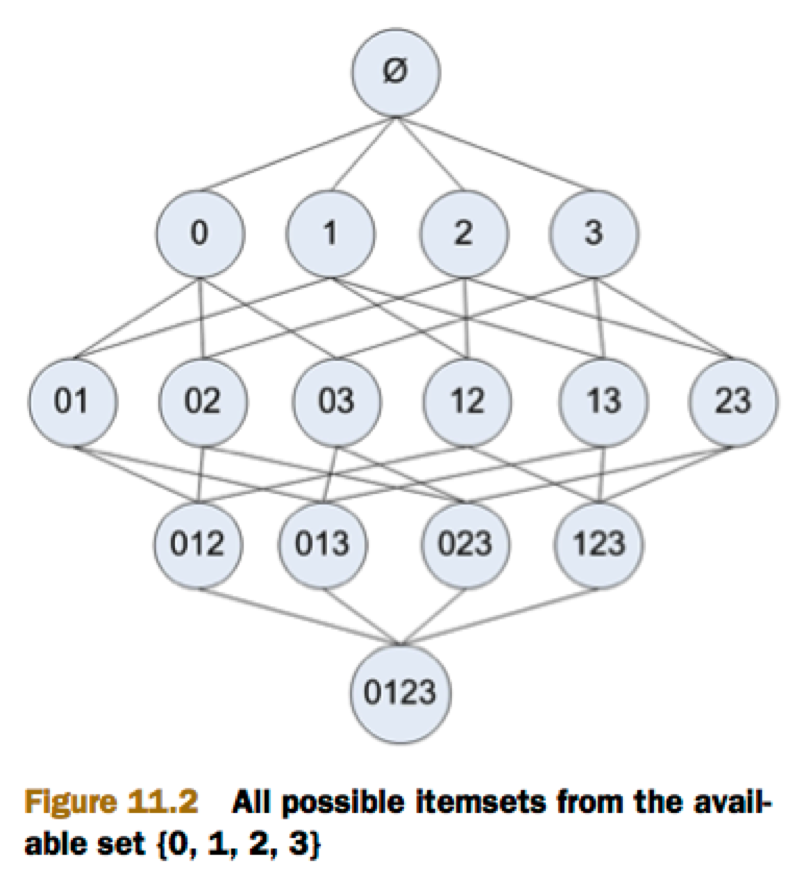
\includegraphics[width=0.75\textwidth]{FullItemsetHierarchy.png}
\caption{\label{fig:allItemsets}[Harrington] }
\end{figure}

We make the following \underline{assumptions} about the itemsets:
\begin{itemize}
\item Ignore the order of the objects, i.e., it doesn't matter which item passed through the checkout counter first.
\item Ignore item count beyond 1 i.e. purchased item count+=1, regardless of quantity purchased 
\end{itemize}

Let's say we are in a store with only $4$ items.  What are the possible combinations of these items?   These are enumerated in Figure \ref{fig:allItemsets}. For each possible itemset size $0\geq k\geq4$ we have $\binom{4}{k}$ possible itemsets. This results in a total of $16$ possibilities.
This seems simple enough, but a store selling merely $100$ items generates $1.26\times 10^{30}$ possible itemsets!

\subsection{The Apriori Algorithm}

There is a simple principle that can help us reduce the computational complexity of this called the \textit{Apriori principle}. The Apriori principle  will help us get what we want and will set the stage for association rule mining.
\par
This term emphasizes the unique origin of this algorithm. This algorithm was devised by data miners (as opposed to data scientists or statisticians). The latter still cringe at the misuse of Latin (it should be ``a priori'') but the original term stuck.

\begin{definition}
The \underline{apriori principle} says that: \newline 1. If an itemset is frequent, then all of its subsets are frequent.  
\newline 2. If an itemset is infrequent, then its supersets are also infrequent.  
\end{definition}

\begin{figure}
\centering
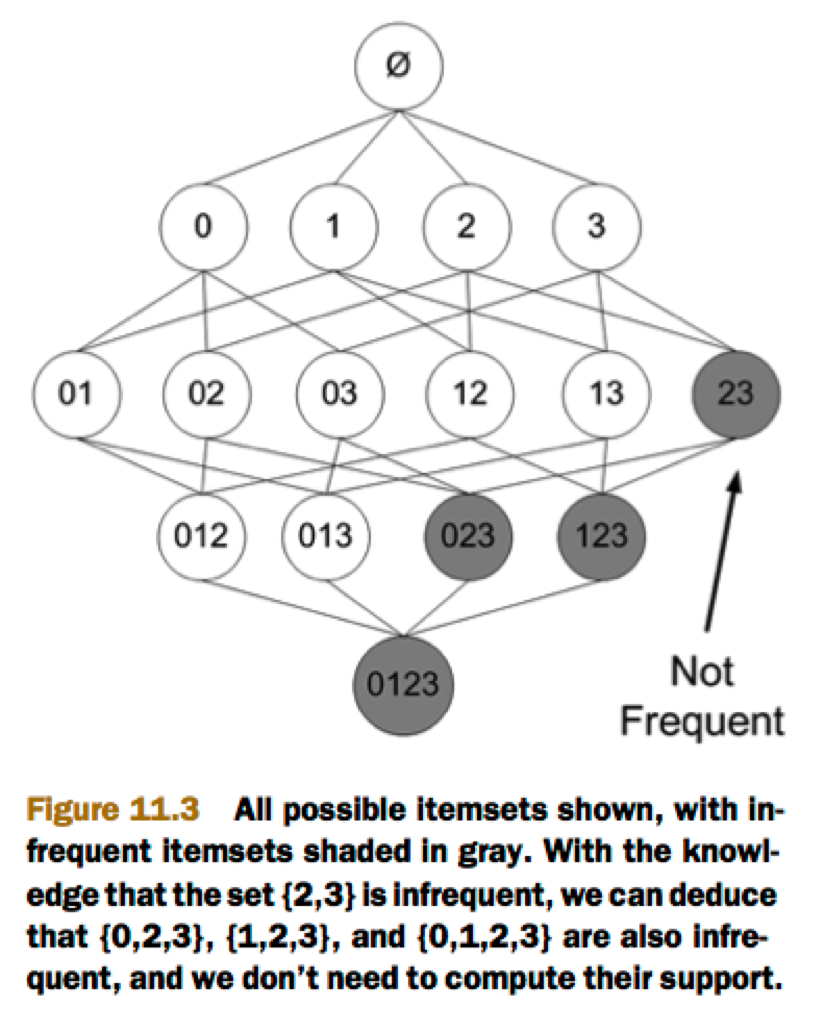
\includegraphics[width=0.75\textwidth]{TrimmedItemsetHierarchy.png}
\caption{\label{fig:trimmedItemsets} [Harrington]}
\end{figure}

Figure \ref{fig:trimmedItemsets} shows an example of the apriori principle in action. If we know that the itemset \{2,3\} is infrequent, i.e., does not meet a given threshold, we don't need to compute the support for of its supersets \{0,2,3\}, \{1,2,3\}, or \{0,1,2,3\} since there is no way they can meet our requirement.

\begin{algorithm}
 \KwData{Dataset D, minimum support level $t$}
 \KwResult{All itemsets in the dataset that have support larger than $t$}
 
  \begin{itemize}
  \item Find all itemsets of size $1$ that have a support level $\geq t$
  \item Combine the surviving itemsets to make itemsets of size $2$
  \item Again, scan through each transaction and discard itemsets that fail to meet the support threshold $t$.
  \item Repeat this procedure as long as there are surviving itemsets (note that the maximum number of possible iterations is the amount of unique items in a basket).
  \end{itemize}
 \caption{Apriori Algorithm}
 \label{alg:apriori}
\end{algorithm}

We use the apriori principle to solve our problem in a way that only requires one pass through the dataset for each itemset size, see Algorithm \ref{alg:apriori}.  The apriori algorithm gives us the list of high support itemsets which we are going to cast into a set of \textit{association rules}. 
\textbf{Worst Case:}Algorithm will iterate through every item in the basket \textbf{Expectation} is that the \textit{Apriori Algorithm} will significantly cut down from a brute force implementation

\subsection{Association Rule Mining}
We use the following notation:
\begin{itemize}
\item $\mathcal{K}$ is an itemset
\item $\forall k\in\mathcal{K}$, $Z_k\in \{0,1\}$ is an indicator for the $k$th item.
\end{itemize}

This model makes the following assumptions:
\begin{itemize}
\item Order of item appearance in set is ignored
\item Item counts above 1 are ignored (i.e. the appearance of an item in a set is the only thing that matters)
\item The Apriori Principle as stated above (if an itemset is infrequent then all of its supersets are also infrequent)
\end{itemize}

The items $k\in\mathcal{K}$ are partitioned into disjoint subsets $A\cup B=\mathcal{K}$ and written:
$$A\Rightarrow B$$
$$\text{``antecedent''}\Rightarrow \text{``consequent''}$$
The support of the rule, denoted $T(A\Rightarrow B)$, is the same as the support of the itemset $\mathcal{K}$ from which it was derived:
$$T(A\Rightarrow B)=support(A\cup B)$$

Think of this as an estimate of observing both itemsets $A$ and $B$ in a randomly selected market basket, i.e., $Pr(A \text{\ and\ } B)$.  We can also define the \textit{confidence}, or \textit{predictability}, $C(A\Rightarrow B)$ of the rule as:
$$C(A\Rightarrow B)=\frac{T(A\Rightarrow B)}{T(A)}$$
Where: 
\begin{itemize}
\item $T(A)$ estimates $Pr(A)$, i.e., $Pr(\prod_{k\in A}Z_k=1)$.
\item The \textit{expected confidence} of the rule is defined as the support of consequent $T(B)$, which estimates $Pr(B)$
\item The \textit{lift} of the rule:
$$L(A\Rightarrow B)=\frac{C(A\Rightarrow B)}{T(B)}=\frac{\text{confidence}}{\text{expected confidence}}$$
\end{itemize}
The lift is an estimate of the association measure $\frac{Pr(A \text{\ and\ } B)}{Pr(A)Pr(B)}$. For random chance the lift equals $1$.\\

{\bf Example}  Given an itemset $\mathcal{K}=\{\text{peanut butter},\text{jelly},\text{bread}\}$, consider the rule $\{\text{peanut butter}, \text{jelly}\}\Rightarrow\{\text{bread}\}$. A support of $0.03$ for this rule means that peanut butter, jelly and bread appeared together in $3\%$ of the market baskets. Confidence of $0.82$ for the rule implies that when peanut butter and jelly were purchased, $82\%$ of the time bread was also purchased. If bread appeared in $43\%$ of all market baskets then the rule would have a lift of $1.95$.

Our goal is to mine association rules $A\Rightarrow B$ with high support and high confidence. The apriori algorithm gives us all the itemsets with high support. We want to find rules with high confidence such that for a given threshold $c$ it holds that: 
$$\{A\Rightarrow B \quad | \quad C(A\Rightarrow B)>c\}$$
An itemset $\mathcal{K}$ of size $|\mathcal{K}|$ has $2^{|\mathcal{K}|-1}-1$ possible partitions into rules of the form $A\Rightarrow (\mathcal{K}-A)$ for a subset $A\subset\mathcal{K}$. A variant of the apriori algorithm can be used to find rules that survive the threshold $c$; see Figure \ref{fig:rules}. The result of this algorithm is a collection of association rules satisfying:
$$T(A\Rightarrow B)>t\quad \text{and} \quad C(A\Rightarrow B)>c$$
All the resulting rules are stored in a database for easy querying.

\begin{figure}
\centering
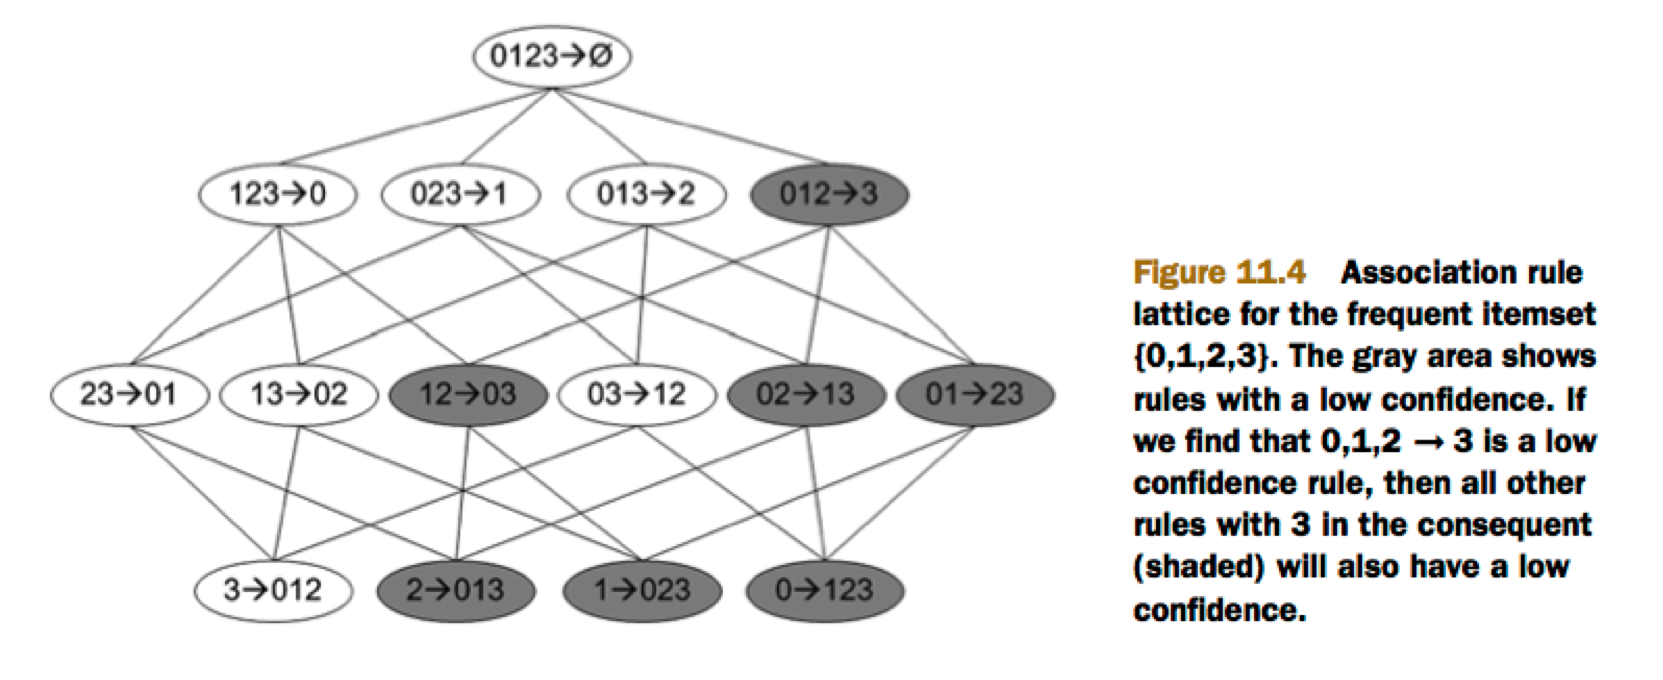
\includegraphics[width=1.0\textwidth]{RuleHierarchy.png}
\caption{\label{fig:rules}[Harrington] }
\end{figure}

{\bf Example} \textit{Display all transactions in which ice skates are the consequent that have confidence over $80\%$ and support of more than $2\%$.}  This would give us insight into items (antecedents) that predicate sales of ice skates.

The advantages of the Apriori Algorithm are that it works on huge datasets and that the rules are easy to interpret. The disadvantage of using the Apriori Algorithm is that rules with high confidence or lift, but low support, are not discovered. 
\newline {\bf For example}, the rule vodka$\Rightarrow$ caviar has high confidence but the consequent, caviar, has very low sales volume (solutions for this situations might include separating to different associative rule sets by price range or adding specific additional models for products that have a high profit margin).

\begin{figure}
\centering
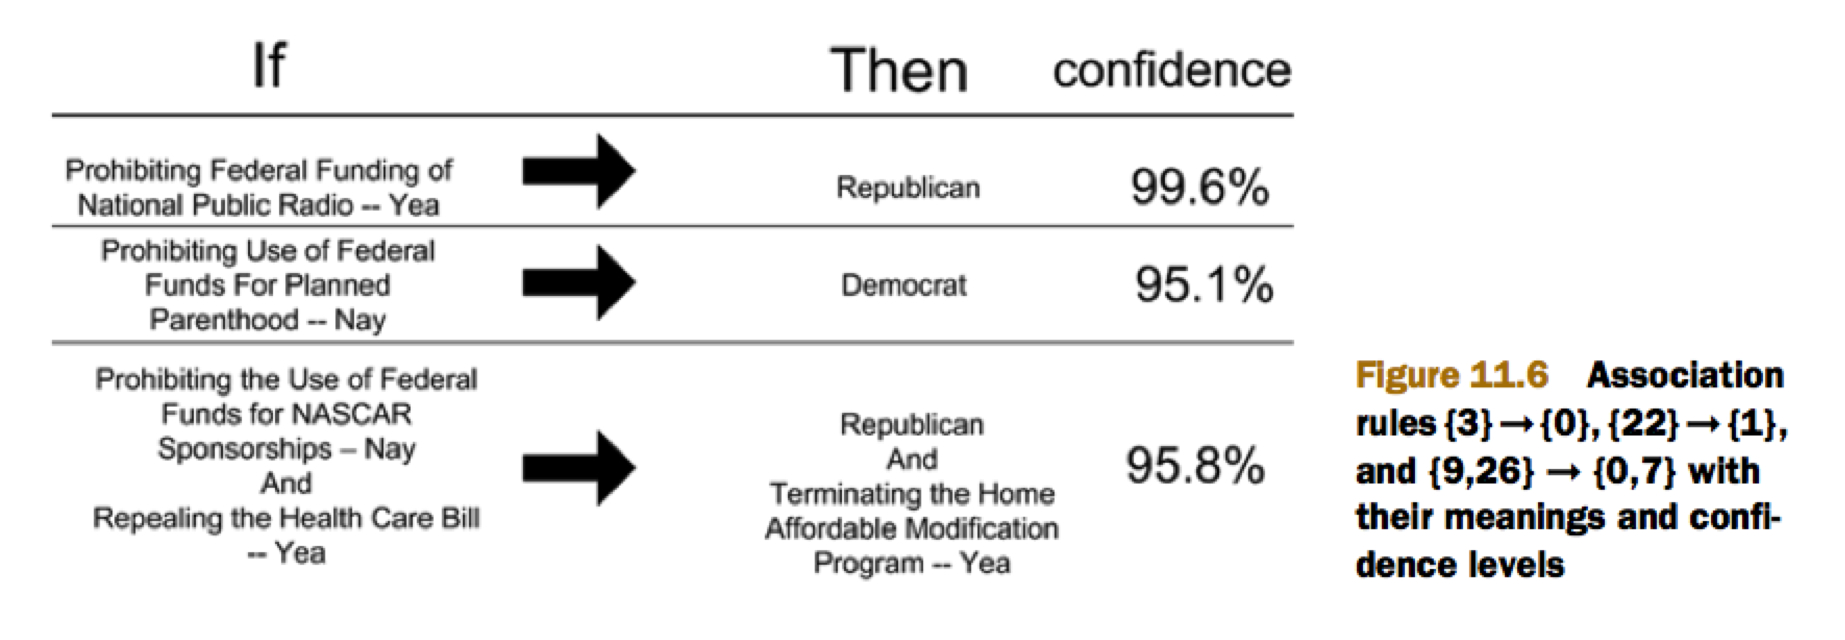
\includegraphics[width=1.0\textwidth]{CongressionalRuleExample.png}
\caption{\label{fig:congressional}[Harrington] }
\end{figure}

Figure \ref{fig:congressional} shows a few sample results from running the Apriori Algorithm on historical congressional voting patterns.

\end{document}
